% !TEX program = xelatex
\documentclass{beamer}
\usepackage{ctex}
\usepackage{graphicx}
\usepackage{hyperref}
\usepackage{booktabs}
\usepackage{tikz}
\usetikzlibrary{arrows.meta, positioning, shapes.misc}

\mode<presentation>
{
  \usetheme{default}
  \setbeamercovered{transparent}
}

\title[AI+Music]{AI+Music 现状、挑战与前沿展望}
\subtitle{新文科人工智能导论 期中报告}
\author{王胤博}
\date{2025 年 10 月 22 日}

\begin{document}

\begin{frame}
  \titlepage
\end{frame}

\begin{frame}{摘要}
  \begin{itemize}
    \item 随着深度学习技术的飞速发展，AI在音乐创作、制作、表演和消费等各个环节都展现出巨大的潜力。
    \item 报告将梳理该领域的主要研究进展、关键技术、代表性公司和应用，并探讨其面临的挑战与未来发展趋势。
    \item 重点将关注AI音乐生成技术的演进，以及其对传统音乐产业带来的深刻影响，并结合前沿研究构想，探讨构建统一音乐智能体的可能性。
  \end{itemize}
\end{frame}

\begin{frame}{目录}
  \tableofcontents
\end{frame}

\section{引言}
\begin{frame}{引言}
  \begin{itemize}
    \item 人工智能与音乐的结合并非全新概念，可追溯至上世纪中叶的“算法作曲”。
    \item 近年来，深度学习和计算能力的突破推动AI音乐从理论走向应用，深刻影响音乐产业。
    \item 本报告旨在系统梳理AI音乐的应用与研究现状、核心技术、产业格局、挑战与未来。
    \item 特别将介绍MUSE (Music Unified State-space Engine) 的构想，展望未来的发展方向。
  \end{itemize}
\end{frame}

\section{AI音乐的发展历程与研究现状}
\begin{frame}{发展历程与研究现状}
  \framesubtitle{早期基于规则和算法的尝试}
  \begin{columns}
    \begin{column}{0.5\textwidth}
      \begin{itemize}
        \item 20世纪50年代起，研究以规则和马尔可夫链等统计模型为主。
        \item 代表作：1957年的《伊利亚克组曲》(Illiac Suite)，由计算机执行音乐规则生成。
        \item 同期贝尔实验室开创了计算机声音合成，为数字音频奠定基础。
      \end{itemize}
    \end{column}
    \begin{column}{0.4\textwidth}
      \begin{center}
        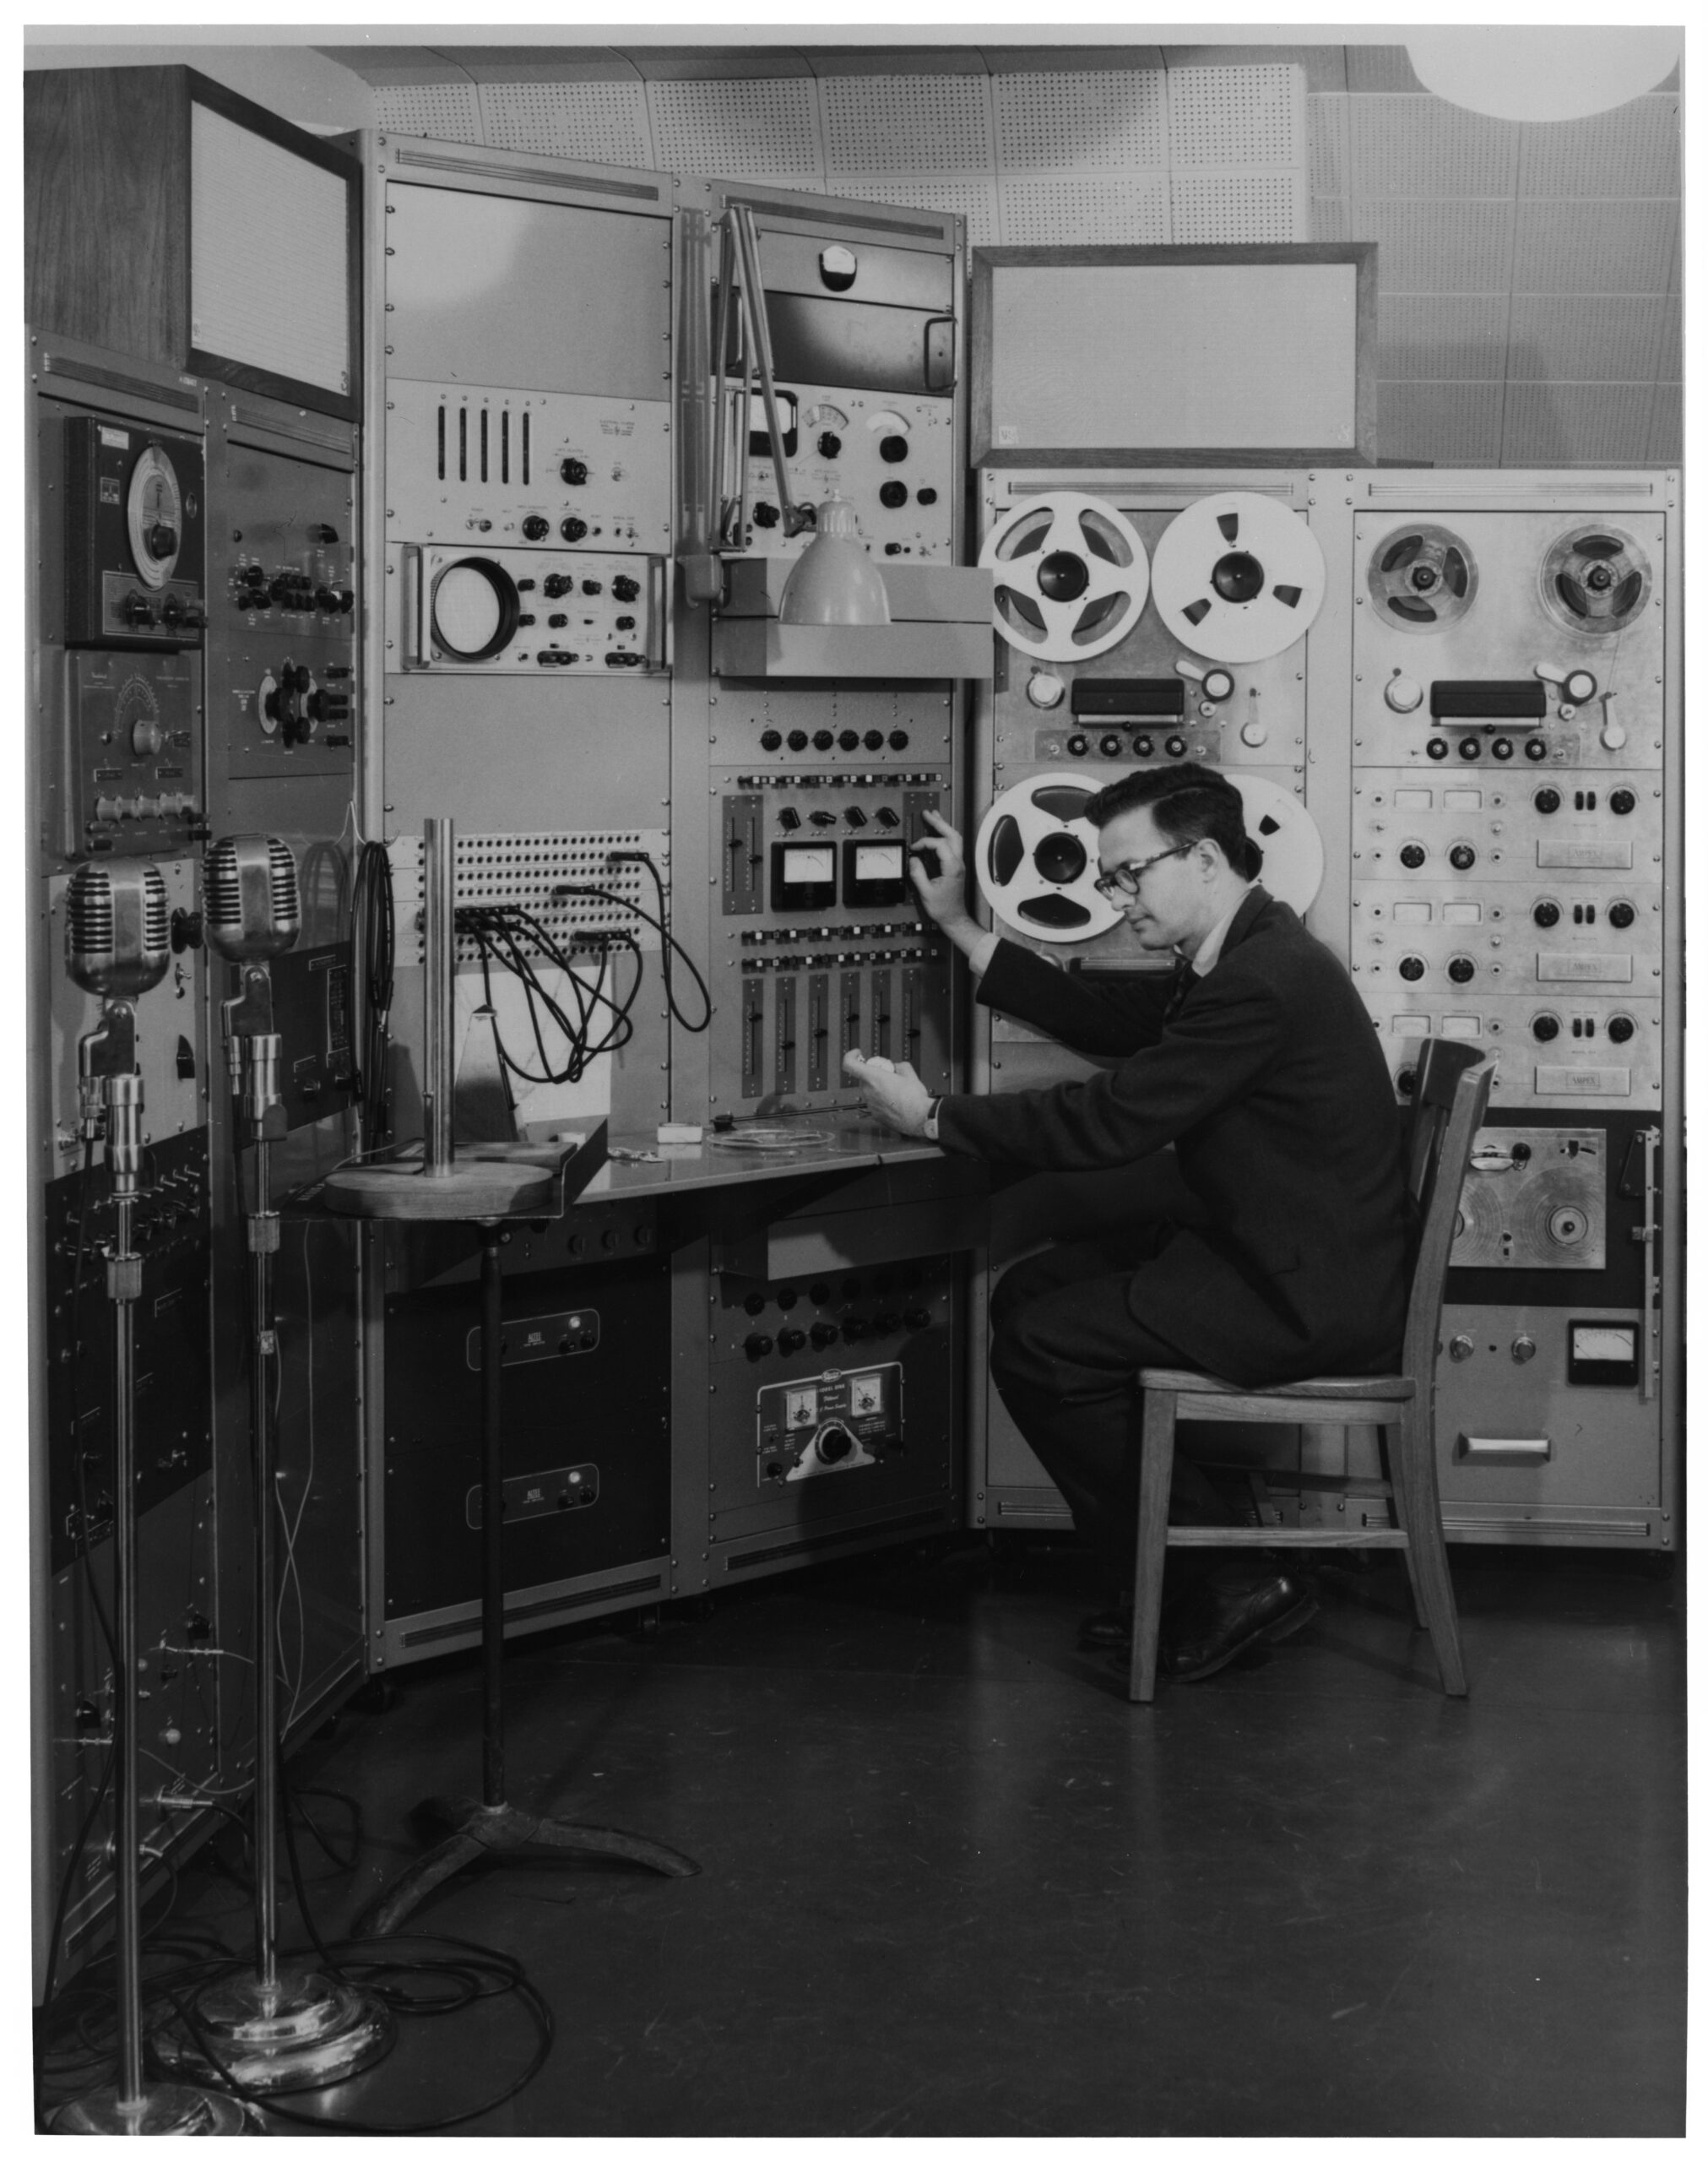
\includegraphics[width=\textwidth]{../figures/Illiac Suite.jpg}
      \end{center}
    \end{column}
  \end{columns}
\end{frame}

\begin{frame}{发展历程与研究现状}
  \framesubtitle{深度学习带来的变革}
  \begin{itemize}
    \item 循环神经网络 (RNN) / 长短期记忆网络 (LSTM) 能有效处理音乐等序列数据。
    \item 生成对抗网络 (GAN) 和 Transformer 等模型进一步提升了生成质量。
    \item 2023年，谷歌MusicLM和Meta的MusicGen成为里程碑式的文生音乐模型。
    \item Suno和Udio在生成带人声的完整歌曲方面取得显著突破。
  \end{itemize}
\end{frame}

\begin{frame}{发展历程与研究现状}
  \framesubtitle{主要研究方向}
  \begin{itemize}
    \item \textbf{音乐生成 (Music Generation)}：创作特定风格、旋律的音乐作品。
    \item \textbf{音乐信息检索 (Music Information Retrieval)}：进行风格分类、情感识别等。
    \item \textbf{音乐语义分析 (Music Semantic Analysis)}：识别音乐表达的语义信息。
    \item \textbf{人机协同创作 (Human-AI Collaborative Composition)}：辅助人类音乐家激发创作灵感。
  \end{itemize}
\end{frame}

\section{核心技术：AI音乐生成模型}
\begin{frame}{核心技术}
  \framesubtitle{主流技术路线}
  \begin{itemize}
    \item \textbf{符号模型 (Symbolic Model)}:
    \begin{itemize}
        \item 处理MIDI等符号化数据，学习乐理规则。
        \item 优点：结构清晰。
        \item 缺点：缺乏真实演奏的表现力。
    \end{itemize}
    \item \textbf{音频模型 (Audio Model)}:
    \begin{itemize}
        \item 直接处理原始音频波形，端到端生成。
        \item 优点：音乐自然流畅，细节丰富。
        \item 代表：MusicLM, MusicGen。
    \end{itemize}
  \end{itemize}
\end{frame}

\begin{frame}{核心技术}
  \framesubtitle{关键模型架构}
  \begin{itemize}
    \item \textbf{RNN / LSTM}：擅长处理序列数据，捕捉时间依赖关系。
    \item \textbf{生成对抗网络 (GAN)}：通过生成器与判别器博弈提升质量，如Hi-FiGAN。
    \item \textbf{Transformer}：凭借并行计算和长序列建模能力成为现代文生音乐的基础架构，如MusicLM、MusicGen。
    \begin{center}
      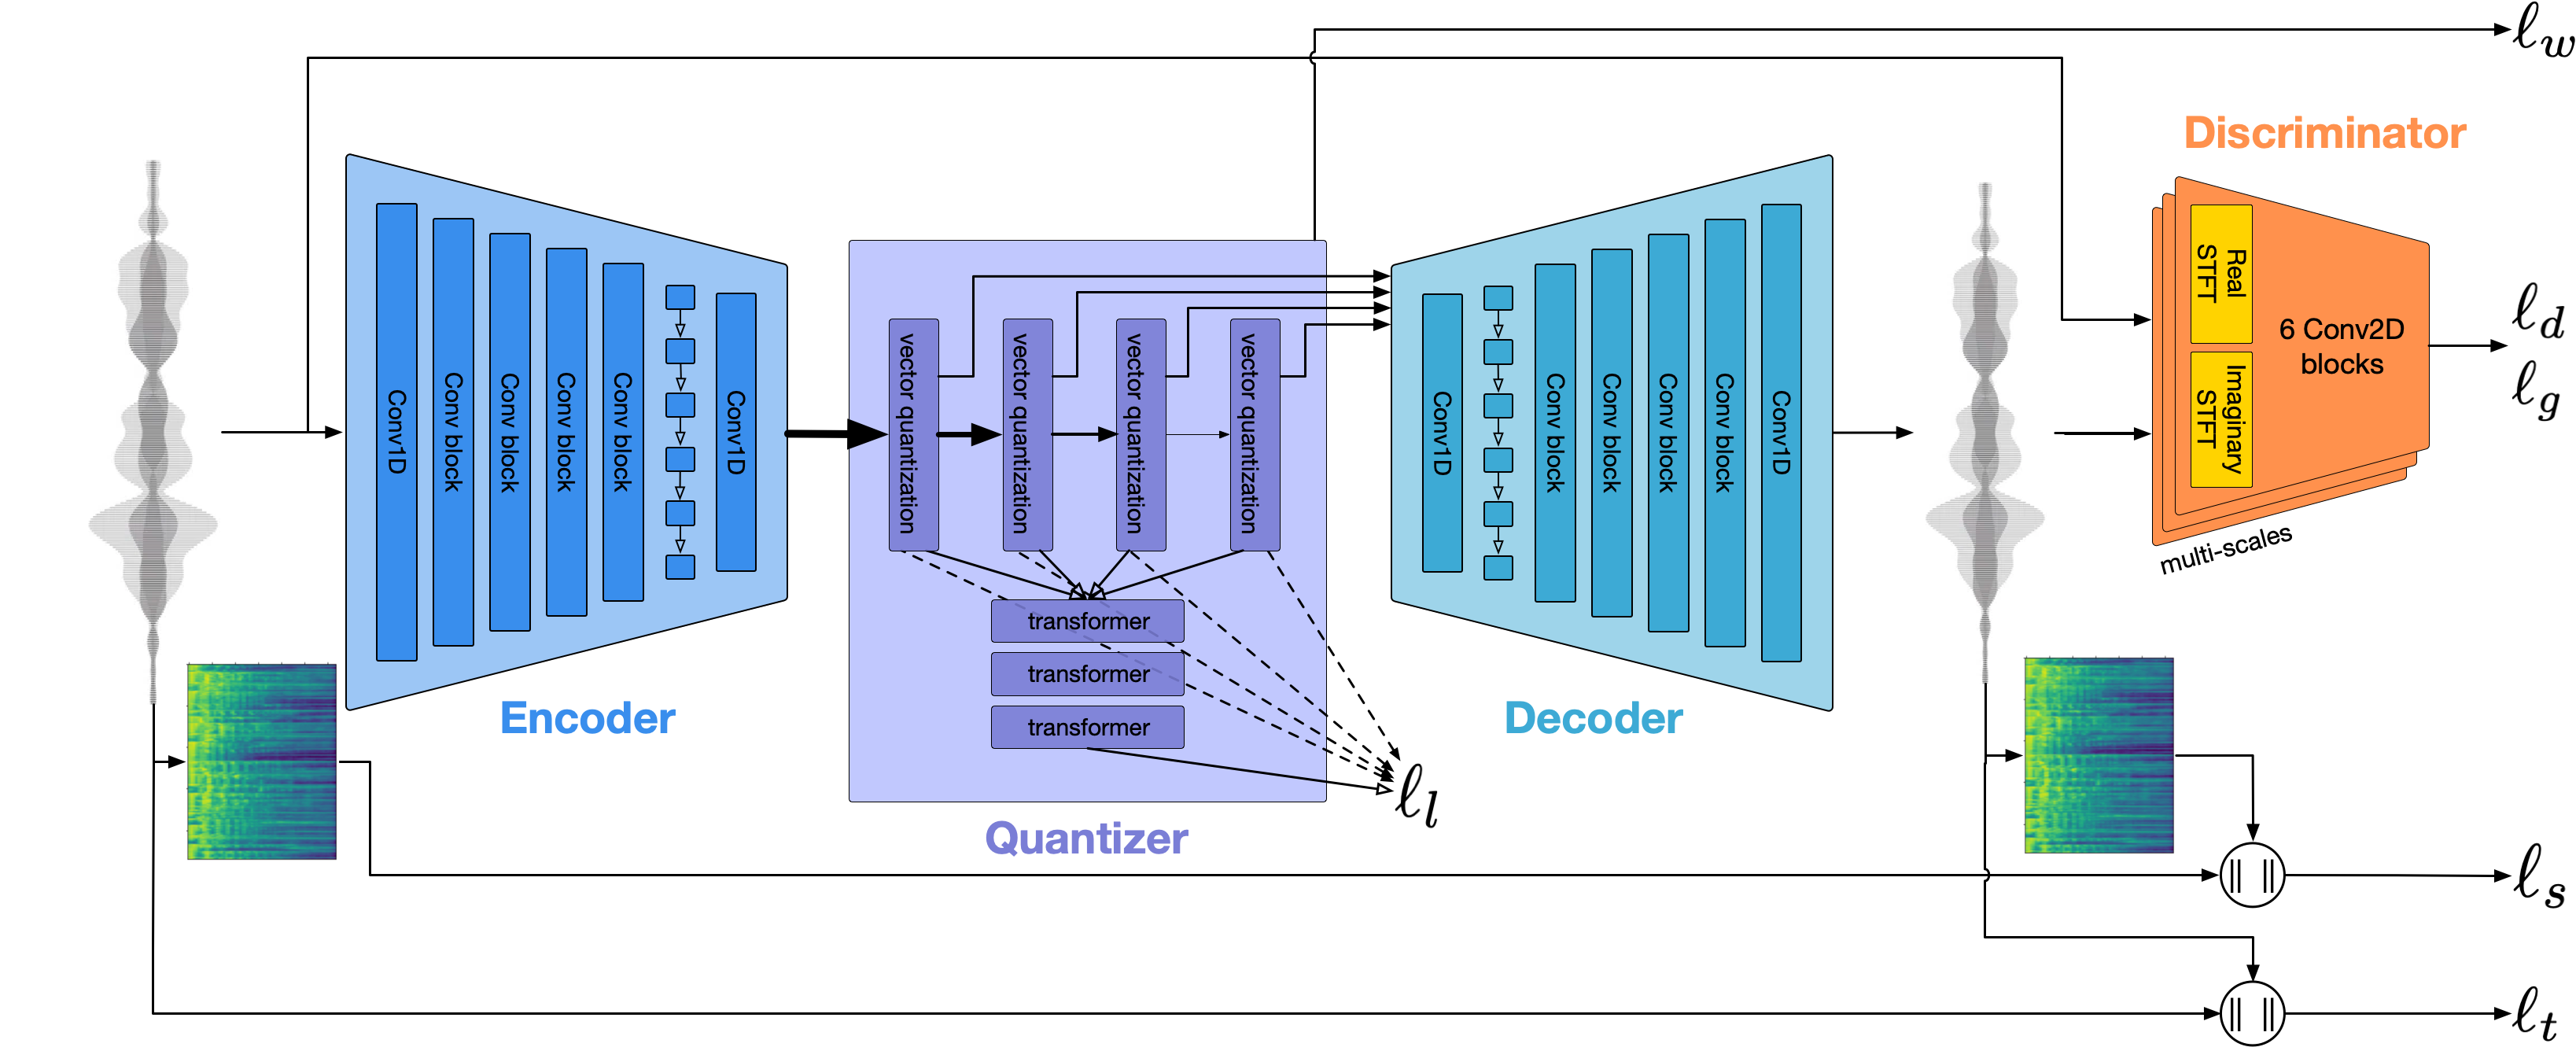
\includegraphics[width=0.5\textwidth]{../figures/EnCodec.png}
    \end{center}
    \item \textbf{扩散模型 (Diffusion Model)}：通过去噪过程生成数据，展现巨大潜力，如AudioLDM。
  \end{itemize}
\end{frame}

\section{产业格局：主要公司与应用}
\begin{frame}{产业格局}
  \framesubtitle{代表性公司和产品}
  \begin{itemize}
    \item \textbf{Suno AI}：AI音乐领域领军者，通过文本提示生成完整歌曲，操作门槛极低。
    \begin{center}
      
\includegraphics[width=0.5\textwidth]{../figures/suno.png}
    \end{center}
    \item \textbf{Udio}：Suno的主要竞争对手，同样专注于文本生成完整歌曲。
    \begin{center}
      
\includegraphics[width=0.25\textwidth]{../figures/udio.png}
    \end{center}
    \item \textbf{Google (MusicLM)} 与 \textbf{Meta (MusicGen)}：科技巨头，在基础研究方面贡献巨大，其模型为领域发展奠定基础。
  \end{itemize}
\end{frame}

\begin{frame}{产业格局}
  \framesubtitle{商业应用场景}
  \begin{itemize}
    \item \textbf{内容创作领域的背景音乐}：为视频、游戏、广告提供快速、低成本、无版权问题的配乐。
    \item \textbf{辅助音乐创作}：为音乐人提供旋律、和声等创作灵感。
    \item \textbf{个性化音乐体验}：根据用户情绪、场景实时生成音乐。
    \item \textbf{音乐教育}：辅助学习作曲和乐理知识。
  \end{itemize}
\end{frame}

\section{挑战与未来展望}
\begin{frame}{挑战与未来展望}
  \framesubtitle{面临的挑战}
  \begin{itemize}
    \item \textbf{版权问题}：核心争议，AI训练数据涉及大量受版权保护作品。大型唱片公司已对Suno和Udio提起诉讼。
    \item \textbf{原创性与艺术性}：AI生成作品的版权归属和艺术价值界定模糊。
    \item \textbf{技术瓶颈与语义割裂}：音乐理解、推荐、生成的模型相互独立，语义空间不统一，导致控制性差、冷启动效果不佳。
  \end{itemize}
\end{frame}

\begin{frame}{挑战与未来展望}
  \framesubtitle{未来发展趋势}
  \begin{itemize}
    \item \textbf{技术与产品的持续迭代}：音质、可控性和多样性将进一步提升。
    \item \textbf{商业模式的成熟与法律框架的完善}：探索新的授权与分润模式，完善相关法律法规。
    \item \textbf{跨学科融合}：与脑科学、认知科学等结合，应用于音乐治疗、情感计算等领域。
    \item \textbf{走向统一模型}：构建打通音乐理解、推荐和生成的统一模型，实现音乐智能闭环。
  \end{itemize}
\end{frame}

\begin{frame}{前沿探索：MUSE (Music Unified State-space Engine)}
  \framesubtitle{动机与核心理念}
  \begin{itemize}
    \item \textbf{目标}：解决音乐理解、推荐、生成系统间的“语义割裂”问题。
    \item \textbf{构想}：构建一个统一的音乐潜空间 (Latent Space)，将三大核心任务融为一体。
    \item \textbf{核心理念}：“好的音乐状态空间”是实现应用闭环的前提，需具备语义充分、结构感知和可控生成三大特性。
  \end{itemize}
\end{frame}

\begin{frame}{前沿探索：MUSE (Music Unified State-space Engine)}
  \framesubtitle{技术方案与架构}
    \begin{center}
      \begin{tikzpicture}[
        node distance=1.5cm and 0.5cm,
        block/.style={rectangle, draw, text width=8em, text centered, rounded corners, minimum height=3em},
        line/.style={draw, -{Stealth}}
        ]
        \node[block] (encoder) {1. 参数冻结的表征编码器 (多模型融合)};
        \node[block, right=of encoder] (fusion) {2. 维度对齐与序列融合};
        \node[block, right=of fusion] (generation) {3. 生成与解码 (DiT + 噪声增强解码器)};
        
        \path[line] (encoder) -- (fusion);
        \path[line] (fusion) -- (generation);
      \end{tikzpicture}
    \end{center}
    
    \begin{itemize}
        \item \textbf{编码器}: 融合自监督、跨模态、结构编码等多种预训练模型，提取丰富特征。
        \item \textbf{融合}: 将异构特征对齐并融合成统一的Latent。
        \item \textbf{生成与解码}: 在Latent上训练扩散模型 (DiT) 进行生成，并通过鲁棒的解码器还原为音频。
    \end{itemize}
\end{frame}

\begin{frame}{前沿探索：MUSE (Music Unified State-space Engine)}
  \framesubtitle{应用闭环展望}
  \begin{itemize}
    \item \textbf{理解与检索}：在潜空间内实现高效的跨模态检索和相似性搜索。
    \item \textbf{推荐系统}：构建基于潜空间的双塔模型，提升推荐质量，解决冷启动问题。
    \item \textbf{生成与编辑}：通过条件化扩散模型，实现对音乐结构和属性的精细可控生成与编辑。
  \end{itemize}
  \vspace{1cm}
  \begin{alertblock}{结论}
    MUSE构想旨在从根本上解决语义鸿沟和可控性难题，是从“模型各自为政”迈向“大一统模型”的探索性思路。
  \end{alertblock}
\end{frame}

\section{结论}
\begin{frame}{结论}
  \begin{itemize}
    \item 人工智能正以前所未有的方式改变音乐的创作、生产和消费模式。
    \item 以Suno、Udio为代表的应用标志着AI音乐已走向大众，并展现出巨大商业潜力。
    \item 尽管面临版权、伦理等挑战，但发展趋势不可逆转。
    \item 未来的发展不仅是生成质量的提升，更在于构建如MUSE构想所描述的，整合理解、推荐和生成的智能闭环。
    \item AI有望成为人类音乐家的创作伙伴，共同开启音乐表达的全新时代。
  \end{itemize}
\end{frame}

\begin{frame}
  \begin{center}
    \Huge Thanks!
  \end{center}
\end{frame}

\end{document}